\documentclass[12pt, conference]{IEEEtran}
\IEEEoverridecommandlockouts
% The preceding line is only needed to identify funding in the first footnote. If that is unneeded, please comment it out.
\usepackage{cite}
\usepackage{amsmath,amssymb,amsfonts}
\usepackage{algorithmic, float}
\usepackage{algorithm}
\usepackage[noend]{algpseudocode}
\usepackage{graphicx}
\usepackage{textcomp}
\usepackage{xcolor}
\usepackage[utf8]{inputenc}
\usepackage[english]{babel}
\usepackage{hyperref}
\usepackage[ruled,vlined]{algorithm2e}


\makeatletter
\newenvironment{breakablealgorithm}
{% \begin{breakablealgorithm}
	\begin{center}
		\refstepcounter{algorithm}% New algorithm
		\hrule height.8pt depth0pt \kern2pt% \@fs@pre for \@fs@ruled
		\renewcommand{\caption}[2][\relax]{% Make a new \caption
			{\raggedright\textbf{\ALG@name~\thealgorithm} ##2\par}%
			\ifx\relax##1\relax % #1 is \relax
			\addcontentsline{loa}{algorithm}{\protect\numberline{\thealgorithm}##2}%
			\else % #1 is not \relax
			\addcontentsline{loa}{algorithm}{\protect\numberline{\thealgorithm}##1}%
			\fi
			\kern2pt\hrule\kern2pt
		}
	}{% \end{breakablealgorithm}
		\kern2pt\hrule\relax% \@fs@post for \@fs@ruled
	\end{center}
}
\makeatother




\urlstyle{same}
\def\BibTeX{{\rm B\kern-.05em{\sc i\kern-.025em b}\kern-.08em
    T\kern-.1667em\lower.7ex\hbox{E}\kern-.125emX}}
\begin{document}

\title{Scheduling Simulator}

\author{\IEEEauthorblockN{ Vineeth Bhat}
\IEEEauthorblockA{\textit{Dept.Computer Science and Engineering} \\
\textit{Frankfurt University of Applied Sciences}\\
Frankfurt, Germany \\
vineeth.bhat@stud.fra-uas.de}
\and
\IEEEauthorblockN{Jathin Sreenivas}
\IEEEauthorblockA{\textit{Dept.Computer Science and Engineering} \\
\textit{Frankfurt University of Applied Sciences}\\
Frankfurt, Germany \\
Jathin.Sreenivas@stud.fra-uas.de}
}

\maketitle

\begin{abstract}
Understanding the working of scheduling algorithms provides us with a knowledge of how to analyse the scheduling of processes, resource utilization, and performance in real-time applications. Various algorithms perform differently and have their unique set characteristics which are advantageous depending on the scenario and application. A simulator enables us to visualize these characteristics, working, and behaviour of scheduling algorithms. By automating the process of scheduling these tasks provided as input and displaying the output intuitively, which reduces the work on creating the schedule and focuses on analysing the behaviour of the scheduling algorithms. This literature focuses on the development of a web application that is machine and platform-independent, with the scope of illustrating multiple scheduling algorithms graphically to help one to draw comparisons and conclusions based on the results.
\end{abstract}


\section{Introduction}
Real-Time systems have wide application and demand in various fields. This is due to the fact that the system provides results or output within a predefined time constraint. Depending on this time constraint the systems can be further classified as Hard real-time systems, that can never miss its deadline and of it misses the deadline the result would be catastrophic. Soft real-time systems, that can miss the deadline occasionally, with an acceptable probability.  Missing of such deadlines would not result in catastrophes.\\
The ability of these systems to meet the deadline depends highly on the scheduler that schedules the tasks and resources for its execution in an optimal way. The scheduler is responsible for the timely execution of tasks, management of resources for the execution, deciding the feasibility of the task. For the operation of this scheduler, various scheduling algorithms fulfill the objective depending on the requirement. 
There can be preemptive and non-preemptive scheduling algorithms. In preemptive algorithms, the task is assigned a specific time-slot and the execution of that task is carried within that time-frame irrespective of the task can be completed or not. If the execution is not completed within the time-frame the execution is interrupted for the next task. Whereas in non-preemptive scheduling the task has to wait for execution till the current task execution is completed.\\
Visualization of the scheduling process by the various algorithm can be done in the form of a graph considering each unit time and the task that is being executed at that time. Considering this idea, this paper presents a solution to simulate various scheduling algorithms and display them in a graphical way for a better understanding of the algorithm.

\section{State of the Art}
There are several real-time scheduling simulators. Majority of these applications display the scheduling process or the feasibility of the tasks for a specific algorithm and are usually executed as a program and the resulting output of the scheduling process is displayed in the console which is difficult to understand how the tasks have been executed during the process, which algorithm executes better. Graphical representation of the execution trace of any algorithm provides us with better information to analyse the behaviour of the algorithm. Even considering this graphical representation, there are only a few simulators that are easily accessible that are implemented using MATLAB or various other platforms, and the majority of which are desktop applications, thereby making them machine-dependent. These simulators tend to focus on one single algorithm at a time and implemented in a specific platform, thereby reducing the flexibility in the system and devoid the user from comparing the execution of various algorithms. Also, the interface to read the inputs and display the output is not intuitive. To develop an application that combines several scheduling algorithms and also provide a user-friendly graphical interface requires a combination of several technologies and good programming skill.\\
Identifying the shortcomings from existing simulators and also considering the requirements that would make the simulator a complete and user-friendly system along with the real-time scenario such as a task might arrive at any given time, this paper focuses on the development of a web-based scheduling simulator. The proposed simulator focuses on the scheduling and execution of tasks provided by the user, using various scheduling algorithms and providing the result of the execution intuitively. The web application provides the flexibility of being machine-independent and provides various options to develop the system and customise to tend to the requirements.\\
One such simulator that is similar to the proposed system is developed using MATLAB, that can be found in the literature \cite{b1}, which focuses on the performance of various scheduling algorithm, also providing the energy consumed by the processor with a good graphical user interface. "Architecture of this simulator is, first it loads the algorithm input that contains various information like execution time, the period for each task. then the algorithm loader loads the implemented algorithm for execution. After which various schedulability tests are performed to analyse the schedulability of the tasks. Once this is completed the performance is evaluated in the performance evaluation module and then the result is displayed in the graphical user interface"\cite{b1}.

\section{Requirements and Analysis}
Considering the usability and the objective of the simulator following functional and non-functional requirements are drawn. This provides an overview of the target the simulator should achieve upon implementation.
\subsection{Functional Requirements}
\begin{itemize}
    \item Users must be able to add, edit, and delete tasks and also its parameters such as period, etc.
    \item Input to the simulator can be uploaded via an excel sheet as well.
    \item Schedulability tests to be performed for each algorithm before the execution.
    \item If a task is not schedulable by an algorithm, the simulator must inform the user.
    \item Simulator must execute all the scheduling algorithms for the same given input at one go.
    \item The implementation of the algorithms must consider the arrival time to replicate the real-time scenario.
    \item Duration of the execution by each algorithm must depend on the LCM calculated using the period of the tasks.
\end{itemize}
\subsection{Non-Functional Requirements}
\begin{itemize}
    \item The simulator must show the visualization of scheduling in a bar graph and line graph by all the scheduling algorithms.
    \item User must be able to hide/view graphs of the algorithms
    \item Easy to use User Interface for changing the parameters of the tasks.
    \item The graphs must be easily understandable
    \item The simulator must show all the graphs of the algorithms at once, to be able to compare the outputs of algorithms
    \item The simulator must allow hiding of a task in the graph, hence a single task alone can be viewed in the graph.
    \item A console log must be displayed on the screen, showing the outputs of the algorithms.
\end{itemize}


\section{Architecture}
The model used for the Simulator is based on the Model-View-Controller architecture (MVC)\cite{b5} using Django Framework as shown in Figure \ref{architecture}. A user request is handled in the following way:
\begin{itemize}
    \item The client enters the necessary tasks and submits on the Web browser which then sends a request for a page to the controller on the server.
    \item The controller retrieves the data it needs from the model, i.e, the scheduling algorithms are triggered, the model takes the input that's required from the controller and performs its execution and then sends the output to the controller, to respond to the request.
    \item The controller gives the retrieved data from the model to the view.
    \item The view is rendered and sent back to the client for the browser to display.
\end{itemize}
In the simulator, the model comprises the implementation of the scheduling algorithms used in the simulator in Python. The controller is the JavaScript file that interacts with the model using JSON. Views are the HTML, CSS, JS files which are used to design the entire web page consisting of graphs, tables, etc.
\begin{figure}
\centerline{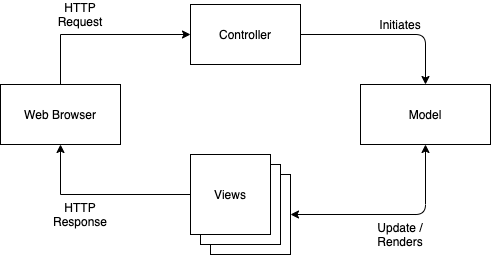
\includegraphics[width=9cm, height=5cm]{RTS_MVC.png}}
\caption{Architecture}
\label{architecture}
\end{figure} 

As shown in the Figure \ref{folderStructure} All the python files are the Model, the Controller is a JavaScript file in the Static/JS folder, the templates, the CSS, other JS files and images all belong to the View.
\begin{figure}
\centerline{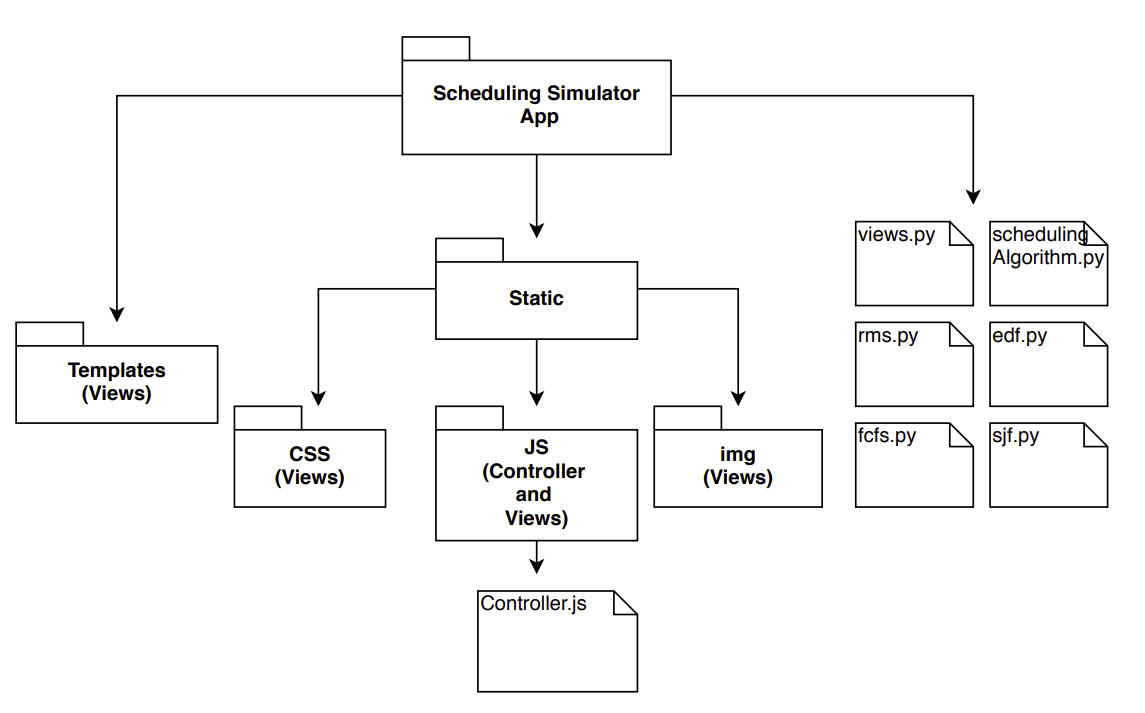
\includegraphics[width=9.5cm, height=6cm]{FolderStructure.png}}
    \caption{File Structure}
\label{folderStructure}
\end{figure}

\section{Class Diagram}
Figure.~\ref{classDiagram} explains the class files and the functions involved in the simulator. The view is a callable that takes a request and returns a response to and from the controller. The view invokes the scheduling algorithm, which is inherited by all the scheduling algorithms implementations. Each of these implementations executes the algorithm for a given input and returns the control to view.

\begin{figure}
\centerline{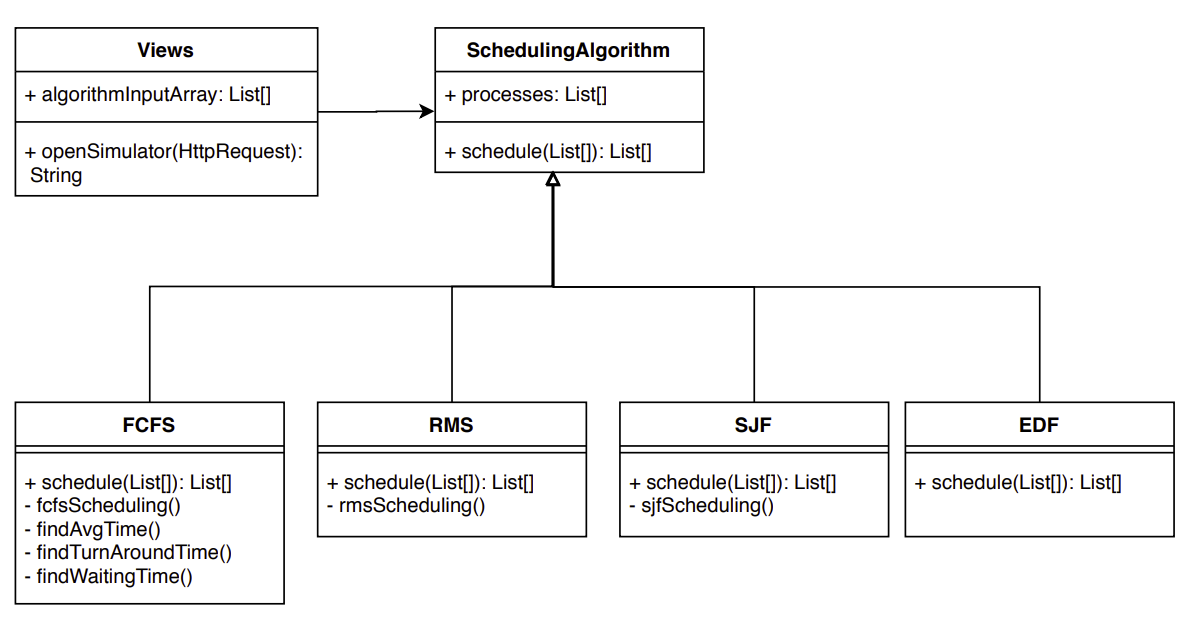
\includegraphics[width=9cm, height=5cm]{ClassDiagram.png}}
\caption{Class Diagram}
\label{classDiagram}
\end{figure} 

\section{Implementation}
As the simulator is a web application, a base HTML is retrieved with no data/graphs when the user first loads the page of the simulator. Figure \ref{layout}, shows the layout of the application. The simulator uses the external CSS libraries of Black Dashboard\cite{b4} to style the web page, a provision is provided for the user to enter the input in a tabular format which is handled by the HTML DOM Table Object in JavaScript. The simulator also uses the CSV libraries to be able to read an excel file as an input. When the user enters the necessary input to the simulator directly to the table on the web page, or user uploads the excel to the simulator and then clicks on submit, on submitting, the Controller is invoked and also certain client-side validations to check the input entered by the user is accurate. The controller that is the JavaScript file, converts this input which is a table structure entered by the user into a JSON in a format which the model understands, and this JSON is sent to the server - Django for processing, Django initially converts this input JSON to Python Objects, and then the models are triggered by passing each model the same input received, now the execution of all the scheduling algorithm takes place, and these models each returns a python object. The model comprises of implementation of all the scheduling algorithms of the simulator, each model returns its output based on the implementation of the algorithm. Django converts these Python objects to JSON and then sends it to the Views. Now the view is rendered using various HTML, CSS, and JS files. Firstly, the JSON is converted to JavaScript objects, and then graphs parameters are generated using JavaScript based on the output given by the model, and then the console is printed which provided a log to the user.  The graphs are designed using the external library Chart.js\cite{b3}, this view along with CSS, and other visualizations are then sent back to the browser to display. \\
\begin{figure}
\centerline{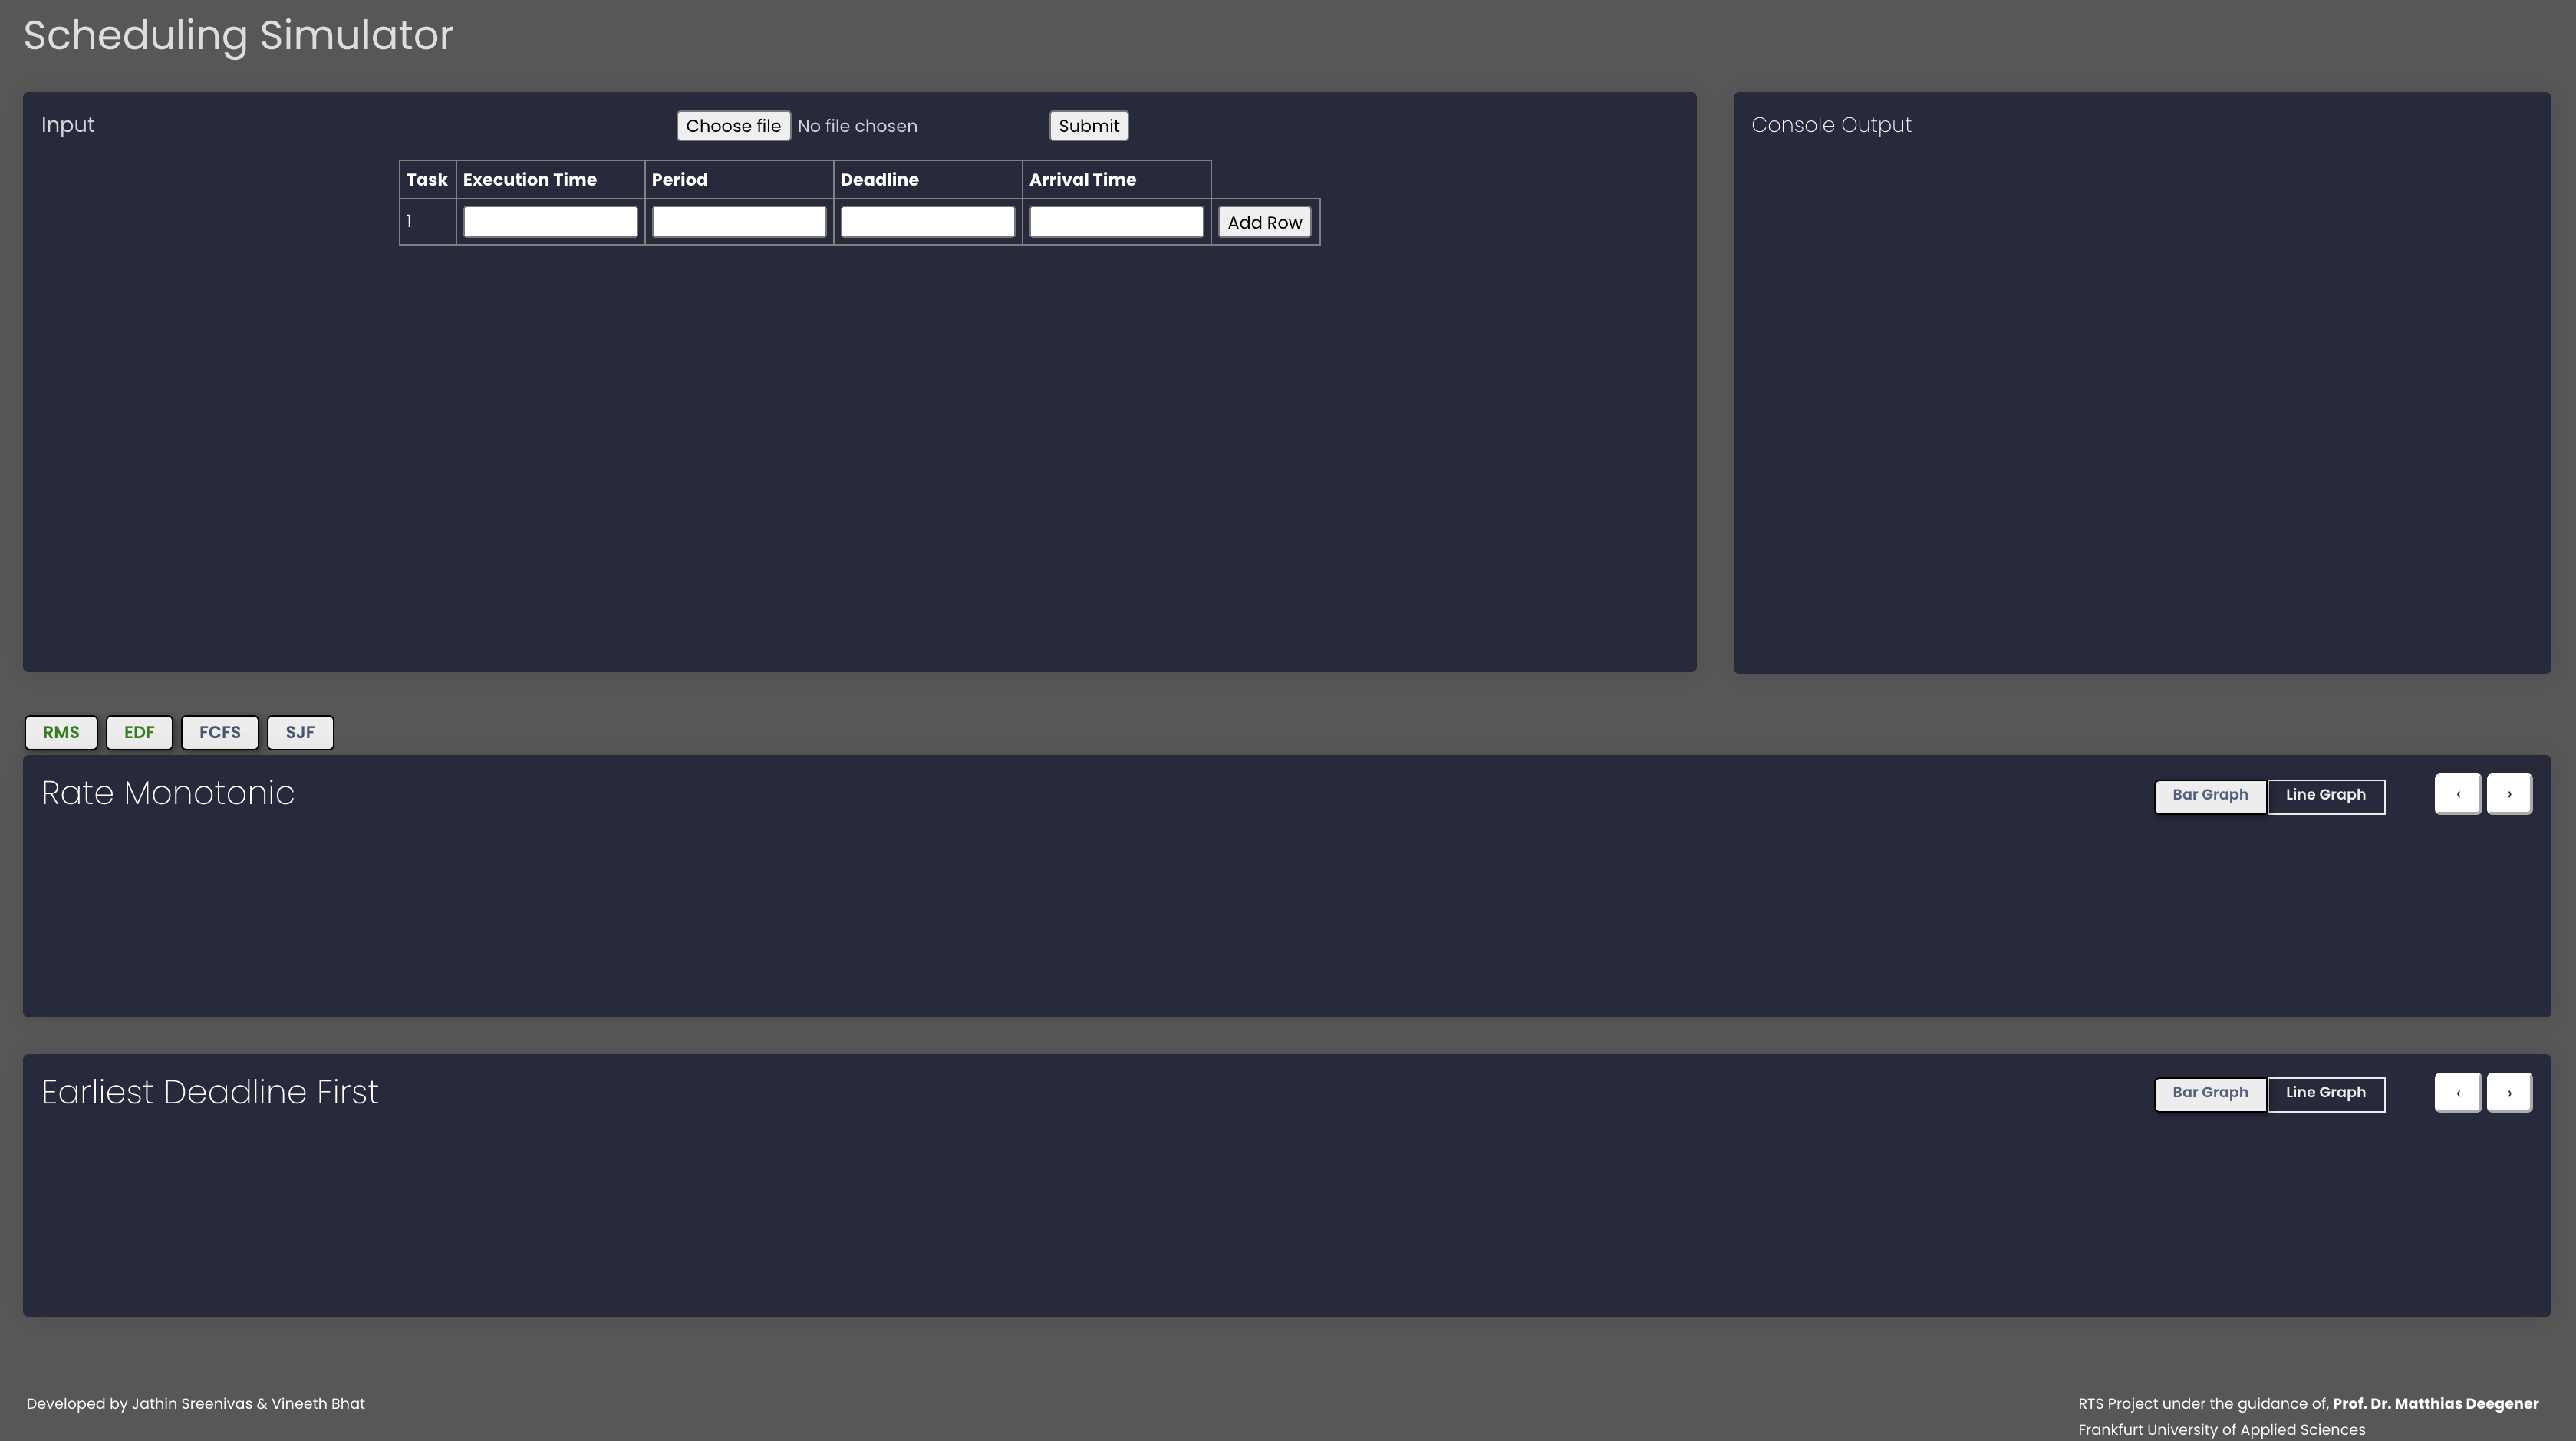
\includegraphics[width=9cm, height=5cm]{layout.png}}
\caption{Application UI}
\label{layout}
\end{figure} 

The implementation of each algorithm in the application is done based on the arrival, period, execution time and also the LCM(range), the application shows the execution of the process for the entire range, that is if a process has an arrival time 0, execution time 5, and period 10. The application considers that this process arrives at every 10 units until the LCM is reached. 

\subsection{Rate Monotonic Scheduling}
Rate Monotonic Scheduling (RMS) is a preemptive based algorithm. It is a priority-based algorithm where a static priority is assigned based on the period. The task with the least period time will have the highest priority. The task with the highest priority will preempt any other process with lower priority. In RMS it is assumed that the deadlines are equal to periods. Resources are not shared between the processes. RMS is one of the most commonly used scheduling algorithms.

\begin{breakablealgorithm}
\caption{Rate Monotonic Scheduling}
\begin{enumerate}
    \item RMS algorithm takes execution time, period, and arrival time as input.
    \item The process is sorted based on period in an increasing sequence. This will set the task with the least period with the highest priority.
    \item Utilization is calculated to verify the schedulability of the tasks. The utilization for a task set with n number of tasks is calculated using,
    \begin{center}
        \begin{equation}
            U = \sum\limits_{i=1}^n \frac{executionTime[i]}{period[i]}
        \end{equation}
    \end{center}
    \item If the utilisation U $\leq$ 1, which is the necessary condition for the algorithm to meet the CPU utilization, then then tasks set can be schedulable. 
    \item The sufficient condition for RMS schedulability is, U \leq $ n(2^{1/n}-1) $. If this condition is not met then the tasks are not schedulable in the current simulator.
    \item A list of all the tasks that need to be executed based on the priority is maintained and this list will contain the execution time of the task, with task number being the index and the value is the execution time and it is updated as the timeline progresses from 0 to LCM.
    \item Once the execution list is updated and if it is not empty, the tasks are executed. The execution time of that task is decremented every time it is executed until it is zero or preempted by another task if that task has higher priority than the current task that is being executed.
    \item This process is repeated until the time reaches the LCM calculated.
\end{enumerate}
\end{breakablealgorithm}
Advantages:
\begin{itemize}
    \item Simple and easy to implement algorithm.
    \item It is optimal compared to other static priority algorithms.
    \item It contains calculated time periods in contrast to other algorithms that neglect the scheduling needs of the tasks.
\end{itemize}
Disadvantages:
\begin{itemize}
    \item It is not optimal in-case of different deadline and periods.
    \item Difficult to support support a periodic and sporadic tasks.
\end{itemize}

\subsection{Earliest Deadline First}
The Earliest Deadline First Scheduling algorithm is one of the fundamental and efficient scheduling algorithms, the priorities of a task are assigned dynamically based on the task's deadline. The EDF algorithm assigns the task with the earliest deadline the highest priority and is executed first. Meaning that the priority of a task is directly proportional to the task's deadline. This is a preemptive algorithm, therefore a currently executing task is preempted whenever another task with the earliest deadline is active. The EDF algorithm works on continuous-time, that is, it assumes that any task can get active at any iteration, so the algorithm selects the task with the earliest deadline at each iteration. \cite{b6}

\begin{breakablealgorithm}
\caption{Earliest Deadline First}
\begin{enumerate}
    \item The parameters arrival time, execution time, period are considered as inputs to the algorithm.
    \item Utilization is calculated to verify if the tasks are schedulable or not. The utilization for a task set with $n$ number of tasks can be calculated using
    \begin{center}
        \begin{equation}
            U = \sum\limits_{i=1}^n \frac{executionTime[i]}{period[i]}
        \end{equation}
    \end{center}
    \item If the Utilization of a task set $>$ 1 (100\%), the tasks cannot be scheduled. 
    \item A  counter is maintained for each task which is initialized to the execution time of the task that is being executed, which is decremented as the time progress.
    \item For each time interval starting from 0
    \item Retrieve the task number which has the earliest deadline (Minimum deadline) from a list of all the deadlines of all the task
    \item If there is already an active task, the current task is paused, and the new task is made active. The current task can resume its executions, only after the new task completes its execution.
    \item The above steps are carried out until LCM.
\end{enumerate}
\end{breakablealgorithm}
Advantages:
\begin{itemize}
    \item One of the most optimal scheduling algorithms.
    \item The algorithm can make the CPU utilization to about 100\% while still guaranteeing the deadlines of all the tasks.
    \item The algorithm produces fewer preemptions in practice, and hence less overhead for context switching.
\end{itemize}
Disadvantages:
\begin{itemize}
    \item The EDF algorithm does not avoid deadline-misses, it can execute a job even though there is not enough time to complete before the deadline.
\end{itemize}

\subsection{First Come First Serve}
The first come first serve algorithm is one of the most simple scheduling algorithms, as the implementation of this algorithm is not complicated, since the only parameter used for scheduling is the arrival time of the process. The algorithm assigns the priority to the process based on the arrival times, the process with the least arrival time is executed first. The algorithm is Non-Preemptive, that is there are no interruptions by other processes, a next process can be started only after the completion of the previous process. Similar to the implementation of the queue data structure. The First Come First Serve algorithm never fails to schedule, it always completed the scheduling successfully.
\begin{breakablealgorithm}
\caption{First Come First Serve}
\begin{enumerate}
    \item The parameters arrival time, execution time, period are considered as inputs to the algorithm.
    \item Based on the period of the process LCM is calculated or the LCM entered on the UI is considered.
    \item The process with the least arrival time is executed first for its execution time.
    \item Once this process completes its execution, the next process with the least arrival time is chosen.
    \item Step 3 and 4 is repeated until the algorithm completes the execution till the LCM.
    \item Waiting time for a process k is calculated using\
        \begin{center}
            waitingTime[k] = executionTime[k-1] + waitingTime[k-1]\
        \end{center} 
    waitingTime[0] = 0, as the first process never waits, its executed as soon as it arrives.
    \item Average Waiting Time can be calculated using, \
        \begin{center}
            averageWaitingTime = totalWaitingTimeForAllProcesses / numberOfProcesses 
        \end{center}
    \item The turn around time for a process k is calculated using,\
    \begin{center}
        turnAroundTime[k] = executionTime[k] + waitingTime[k]
    \end{center}
    \item Total Turn Around Time is calculated using,\
    \begin{center}
        averageTurnAroundTime = totalTurnAroundTimeForAllProcesses / numberOfProcess
    \end{center}
\end{enumerate}
\SetAlgoLined
\end{breakablealgorithm}
Advantages:
\begin{itemize}
    \item Simplest Scheduling Algorithm.
    \item Implementation not complicated.
    \item First come First Served and allows the task to complete its execution, there is no need for any preemptions.
\end{itemize}
Disadvantages:
\begin{itemize}
    \item As the algorithm is Non Preemptive, the average waiting time is very high.
    \item Short processes that are at the back of the queue have to wait for the long process at the front to finish.
    \item No Concurrent process execution.
    \item FCFS is not very efficient.
\end{itemize}

\subsection{Shortest Job First}
The shortest job first can be preemptive and non-preemptive. Preemptive is where the execution of a task can be interrupted by another task that has the least execution time than the one that is being executed. Whereas in a non-preemptive algorithm the task with shortest execution time is executed till its completion. The application implements the non-preemptive version of the algorithm. Following steps explains the steps involved in scheduling the tasks based on the shortest job first,
\begin{breakablealgorithm}
\caption{Shortest Job First}
\begin{enumerate}
    \item Tasks are sorted based on the execution time with the least execution time at the beginning of the order.
    \item For each time point starting from 0, if a task or multiple tasks has arrived execution time of those tasks is added to an execution list.
    \item Task with minimum execution time is considered for execution and the period is updated based on the arrival time. Also, the execution time of that task in the execution list is updated, so that it is not considered for further execution.
    \item A counter is maintained which is initialized to the execution time of the task that is being executed, which is decremented as the time progress, and once the execution is completed the next task with least execution time is picked up for execution.
    \item The process is repeated till the LCM of execution time which is calculated earlier.
\end{enumerate}
\end{breakablealgorithm}
Advantages:
\begin{itemize}
    \item Shortest jobs are executed early, there by maximizing the throughput. It is possible to complete more tasks in the given time.
    \item Algorithm provides optimal average waiting time for the tasks scheduled.
\end{itemize}
Disadvantages:
\begin{itemize}
    \item Possibility of starvation if shortest jobs keep occurring. That cases the tasks with larger execution to wait indefinitely.
    \item Not possible to implement this at short term CPU scheduling level.
\end{itemize}


The output of all the scheduling algorithms which will be in the form of two-dimensional arrays including each time unit till the LCM calculated and corresponding execution trace of each task for that time is returned to the views as described.


\section{Development Environment}
Following list of technologies are used along with certain external libraries for the development of this simulator.\\
Technologies used:
\begin{itemize}
    \item Django Framework (Python 3)
    \item JavaScript
    \item HTML
    \item CSS
    \item JSON
\end{itemize}
External Libraries Used:
\begin{itemize}
    \item JavaScript: Chart.js \cite{b3}
    \item CSS: Black Dashboard \cite{b4}
\end{itemize}

This application is developed using Django Framework, which is a Python-based open-source web framework, that follows the Model-View-Controller (MVC) architectural pattern. This provides good support for the integration of GUI using HTML, CSS, and JavaScript which forms the core component of the UI. For displaying the scheduling outputs as graphs animatedly and interactively, Charts.js is used which is an open-source community project for rendering charts, graphs using JavaScript.\cite{b3} The styling, which is a color font, the layout of the front-end of the application is developed with the help of Bootstrap, which is an open-source front-end framework. \cite{b4}\\

Following tools and softwares were incorporated to carryout the development process.\\
Tools and Softwares used:
\begin{itemize}
    \item IDE: PyCharm
    \item Version Control: GitHub
    \item Browser: Chrome, Safari
    \item Documentation: Overleaf (LaTeX)
\end{itemize} 
PyCharm was the Integrated Development Environment(IDE) used for the development, which is a dedicated IDE by JetBrains for the development of Python. To maintain the collaboration within the team, GitHub was used as the version controlling tool. The development was mainly tested and executed in the Chrome browser and also in Safari. Documentation is done in Overleaf, which is an online LaTeX editor.\\



\section{Discussions}
The simulator provides various features to make the application intuitive and user friendly. As shown in Figure \ref{layout}, the layout is divided into different sections. Input section as displayed in Figure \ref{inputSection} in the screen takes the input, here the "Choose file" button is used to upload the .csv file, which will be added to the table below upon selection. The edit button allows the user to edit the input and later save it before submitting it. Similarly, a task can be deleted using the delete option. Add provides the user with an option to add additional tasks below the existing tasks.
\begin{figure}
\centerline{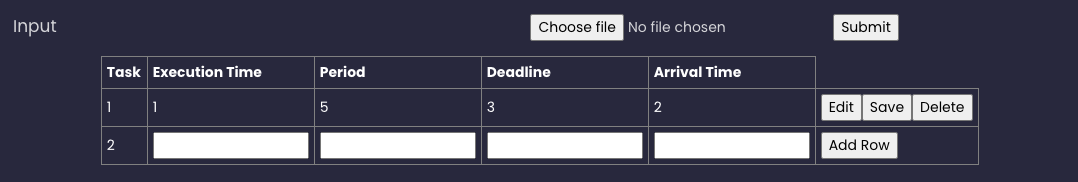
\includegraphics[width=9cm, height=1.75cm]{inputDiscussion.png}}
\caption{Input Section}
\label{inputSection}
\end{figure} 
Figure \ref{console} shows the console that displays the output in the form of texts. That is displaying the inputs, timeline length, schedulability of the process are displayed. 
\begin{figure}
\centerline{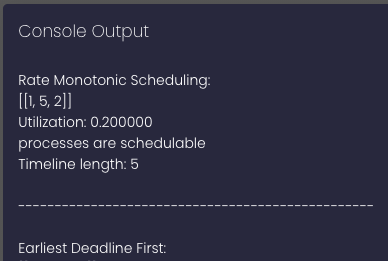
\includegraphics[width=8cm, height=4cm]{outputDiscussion.png}}
\caption{Console Log Section}
\label{console}
\end{figure} 
\begin{figure}
\centerline{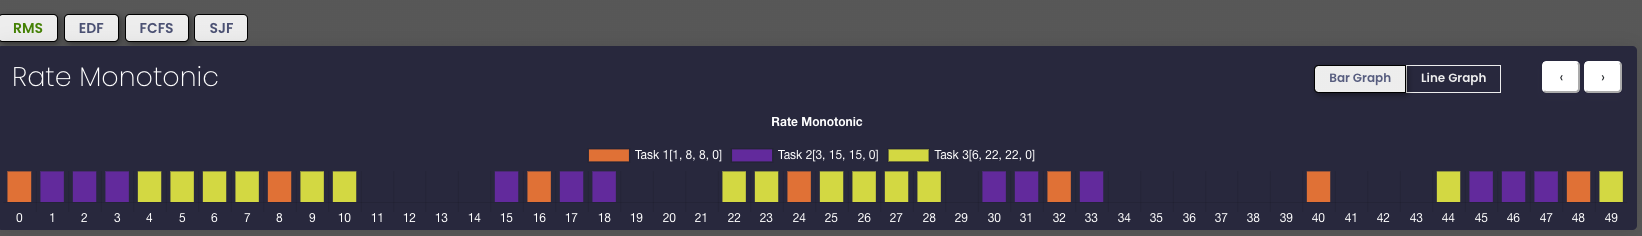
\includegraphics[width=9cm, height=1.5cm]{barGraphDiscussion.png}}
\caption{Graphs Section}
\label{graphs}
\end{figure} 
The buttons RMS, EDF, FCFS, and SJF displayed in Figure \ref{graphs} allows the user to select the algorithm whose output is displayed below. If a particular algorithm is selected for example RMS then the letters RMS is highlighted in green and if an algorithm is not selected its letter will not be highlighted. The button "Bar-Graph/Line-Graph" within each of the scheduling algorithm sections which displays the execution trace in the form of a bar-graph by default lets the user switch between bar-graph or line-graph. Similar to earlier buttons the graph selected for displaying the output will be highlighted.
\begin{figure}
\centerline{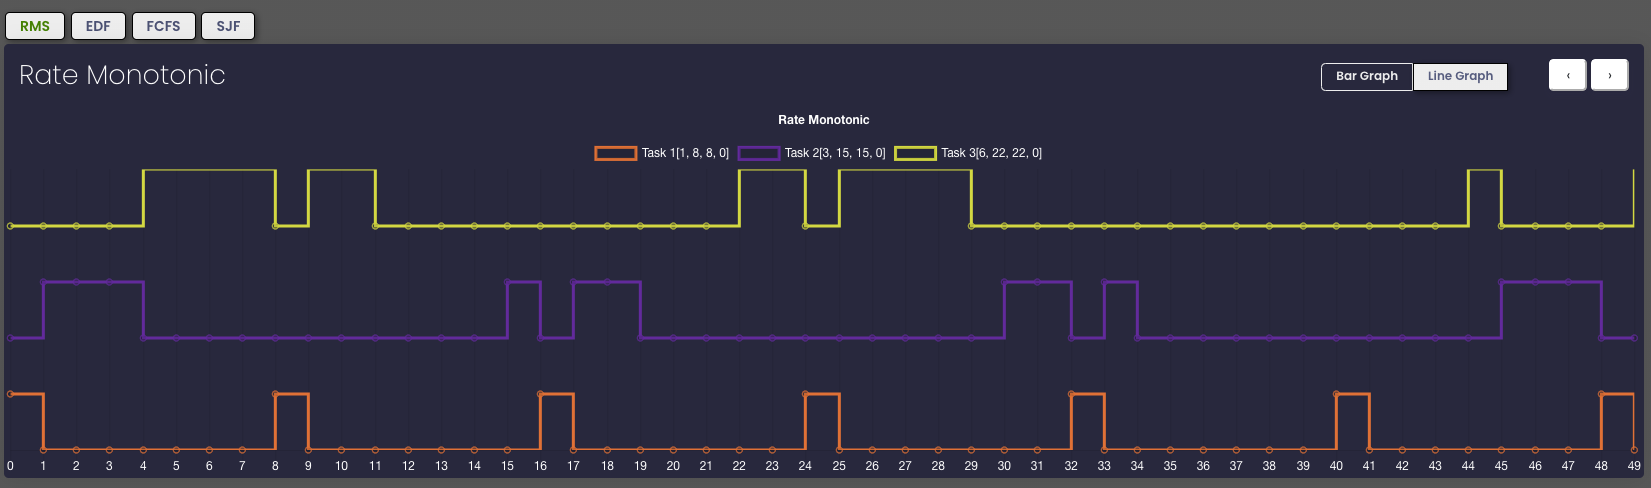
\includegraphics[width=9cm, height=3cm]{lineGraphDiscussion.png}}
\caption{Line Graph}
\label{lineGraphs}
\end{figure} 

The navigation arrow at the end allows the user to move along the timeline in increments of 25 in either direction. In the graph section the timeline is shown along the X-axis as displayed in Figure \ref{graphs}. Each task will be assigned a unique color which is displayed at the top of the graph section for each algorithm along with task number and inputs. For bar-graph, at any given time if a task is being executed then a bar of unit length of respective color is displayed. If none of the tasks are being executed then that time frame will be empty. Whereas the line-graph provides an individual line for each task with unique color stacked one above the other as shown in Figure \ref{lineGraphs}. For any given time if a task is being executed then the respective task will show a step, if not then the line will remain flat.

\subsection{Validations and Constraints}
Certain validations and checks are provided to avoid fatal errors during the execution. Also, there exist certain limitations in the application that prevent the user from performing normal operations.
\begin{itemize}
    \item While providing input through the fields provided on the screen, the user cannot add a new row without completely filling all fields in that row.
    \item If a row in empty in the uploaded .csv file as input, then that row is skipped and the next row if exists then selected.
    \item The order of input in the .csv file should follow the order displayed on the screen. That is for a task the file should contain the inputs in the order of Execution Time, Period, Deadline, and Arrival Time. Similarly for any subsequent tasks follows the previous row.
    \item All the input fields are numeric fields.
    \item If an input field is edited by the user, it should be saved before clicking submit.
\end{itemize}

\section{Results}
 The application was tested with various scenarios by considering several combinations of inputs. One such case is given in table \ref{tab:input} which illustrates the result created by the simulator also describes the difference between execution by the different algorithm can be clearly identified as the comparison between the execution of multiple scheduling algorithms being one of the main features of this simulator.
 
\begin{table}[]
    \centering
    \caption{Input - I}
    \label{tab:input}
    \begin{tabular}{|c|c|c|c|c|}
    \hline
        Task & Execution Time & Period & Deadline & Arrival Time  \\
    \hline
         1 & 1 & 8 & 8 & 2 \\  
         \hline
         2 & 2 & 22 & 22 & 1 \\
         \hline
         3 & 3 & 15 & 15 & 0 \\
         \hline
    \end{tabular}
\end{table}


\subsection{Rate Monotonic Scheduling}
Considering the input from table \ref{tab:input}, RMS assigns the priority based on the least period of the task among the task set. Here at a time, t = 0 only task T3(Yellow) is available, hence it will have the least period that is 15, it will be executed as shown in Figure \ref{Output_RMS}. At t = 1, T2(Purple) arrives with period 22, so it will have lower priority than T3, T3 will not be preempted and will continue its execution at time t = 1.  At t = 2, T1(Orange) arrives with period 8 which is the least of the three tasks available hence it will have the highest priority and it will interrupt the execution of T3. The execution time of T1 is 1 so it will be executed only once at t = 2. This will allow the task with the next highest priority to execute which is T3. T3 has already completed 2 execution cycle out of 3, it will now execute once at t = 3 and allows T2 to execute. T2 was not allowed to execution by T1 and T3 earlier will execute at time t = 4 and 5. By t = 5, all tasks have been executed once within the given period. The next period is of T1 which will arrive at t = 10, till that time there will be no task to execute as the other tasks have a much higher period of execution. At t = 10, T1 is again executed once and this process of execution repeats for all the tasks till the timeline ends.
\begin{figure}
\centerline{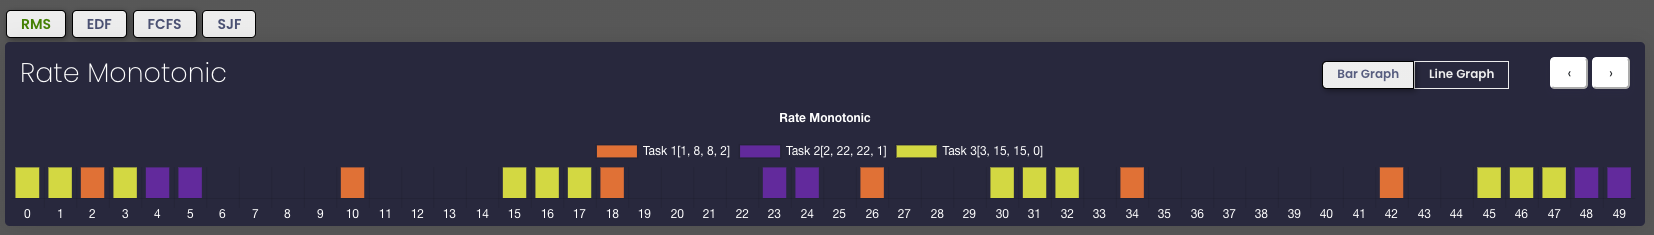
\includegraphics[width=9.25cm, height=1.5cm]{Output_RMS.png}}
\caption{Rate Monotonic Scheduling}
\label{Output_RMS}
\end{figure} 

\subsection{Earliest Deadline First}
The EDF scheduling algorithm is a preemptive scheduling algorithm, which gives the highest priority to the task with the earliest deadline. Based on the input given in table \ref{tab:input}, the algorithm schedules these tasks as shown in Figure \ref{Output_EDF}. At time t = 0, as only Task T3(Yellow) is available, T3 is executed. At t = 1, T3 and T2(Purple) are available and since T3 has the earliest deadline T3 is executed; at this point, both T2 and T3 haven't completed their execution, so both the tasks are active. At t = 2, T3, T2 \& T1(Orange) are available, now T1 has the earliest deadline, hence T1 is executed and T1 has completed its execution (Execution Time = 1) so T1 is no longer active. At t = 3, only T2 and T3 are available, and T3 has the earliest deadline hence T3 is executed, now T3 has completed its execution and now T3 is no longer active. At t = 4 and 5, only T2 is available, and T2 is executed. At t = 6 to t = 9, None of the tasks are active. At time t = 10, the period of T1 is 8, T1 is active, and hence this task is executed, and this process of execution repeats for all the tasks till the timeline ends.
\begin{figure}
\centerline{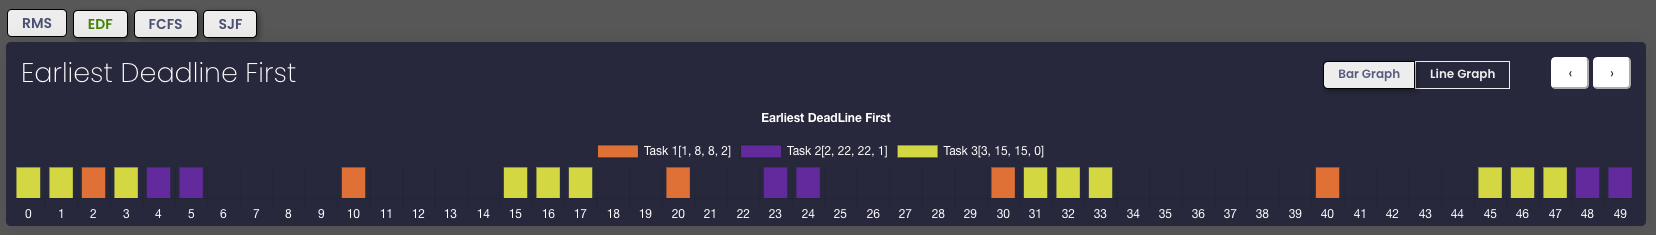
\includegraphics[width=9.25cm, height=1.5cm]{Output_EDF.png}}
\caption{Earliest Deadline First Scheduling}
\label{Output_EDF}
\end{figure} 


\subsection{First Come First Serve}
The FCFS scheduling algorithm is a non-preemptive algorithm, which gives the highest priority to the task which arrives first. Based on the input given in table \ref{tab:input}, the algorithm schedules these tasks as shown in Figure \ref{Output_FCFS}. At time t = 0, only Task T3 has arrived and active, since its execution time is 3, from t = 0 to t = 2 T3 is executed completely and therefore T3 is no longer active. At t = 3, T1 with arrival time = 2 and T2 with arrival time = 1 are active, since T2 arrived before T1, T2 (Execution time = 2) is executed from t = 3 to t = 4. At t = 5, only T1 is active, T1 is executed. The next period is of T1 which will arrive at t = 10, till that time there will be no task to execute. At t = 10, T1 is again executed once and this process of execution repeats for all the tasks till the timeline ends.

\begin{figure}
\centerline{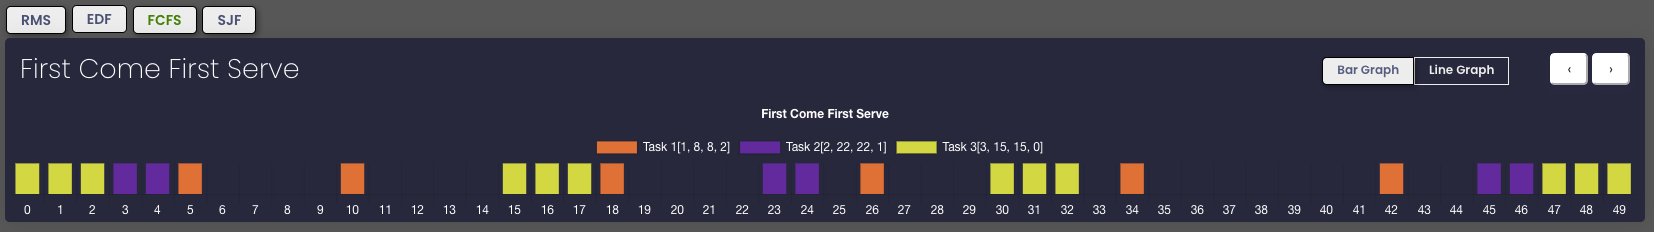
\includegraphics[width=9.25cm, height=1.5cm]{Output_FCFS.png}}
\caption{First Come First Serve Scheduling}
\label{Output_FCFS}
\end{figure} 


\subsection{Shortest Job First Scheduling}
The non-preemptive Shortest Job First scheduling algorithm, assigns priority based on the least execution time. For the input in table \ref{tab:input}, at time t = 0, task T3(Orange) is the only available task for execution and it will be executed immediately as it is the one with the shortest job as shown in Figure \ref{Output_SJF}. At t = 1, T2(Purple) arrives with smaller execution time but this is a non-preemptive algorithm hence the task that is currently being executed, T3 will continue its execution till it is completed. At t = 2, T3 is completed, and also T1(Orange) is available along with T2. Of these two tasks, T1 has the shortest execution time hence it is picked for execution at t = 3. Since the execution time of T1 is 1 it is completed at t = 3 and the next task T2 is executed at t = 4 and 5. Till time t= 10, there will no task for execution as the next earliest period is of T1 at t = 10. This process is repeated until the timeline ends.\\
\begin{figure}
\centerline{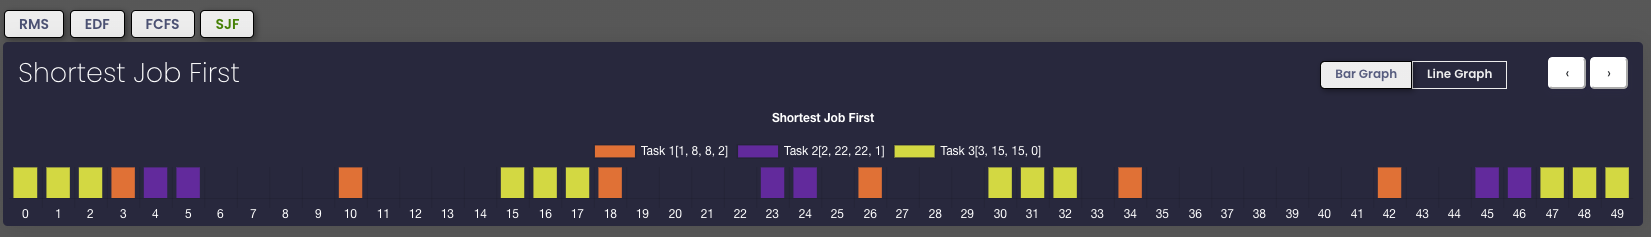
\includegraphics[width=9.25cm, height=1.5cm]{Output_SJF.png}}
\caption{Shortest Job First Scheduling}
\label{Output_SJF}
\end{figure} 

Displaying all these results together as shown in Figure \ref{comparison}, will enable the user to compare multiple algorithms or choose which algorithms to display thereby showing the clear differences in execution between various scheduling algorithm.\\

\begin{figure}
\centerline{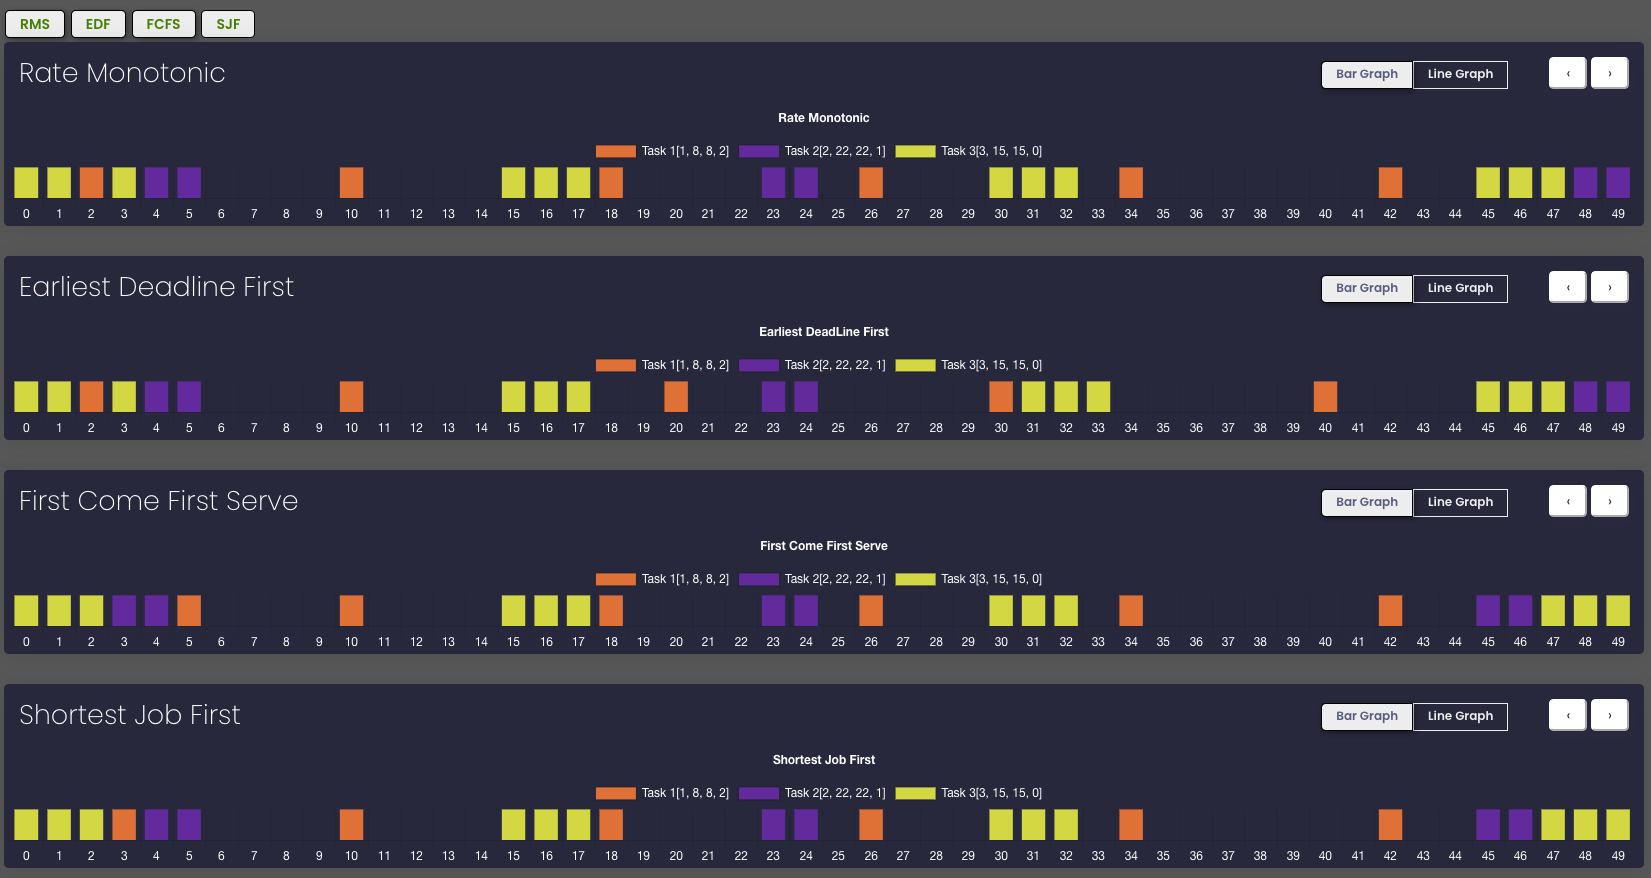
\includegraphics[width=9cm, height=7cm]{Output.png}}
\caption{Comparison of different scheduling algorithms - Input I}
\label{comparison}
\end{figure} 

\begin{table}[]
    \centering
    \caption{Input II}
    \label{tab:input2}
    \begin{tabular}{|c|c|c|c|c|}
    \hline
        Task & Execution Time & Period & Deadline & Arrival Time  \\
    \hline
         1 & 5 & 25 & 25 & 5 \\  
         \hline
         2 & 5 & 30 & 30 & 0 \\
         \hline
         3 & 6 & 25 & 25 & 0 \\
         \hline
         4 & 7 & 20 & 20 & 1 \\
         \hline
    \end{tabular}
\end{table}


\subsection{Handling of Non-Schedulable Tasks}
A second example is the one where the algorithm fails to schedule the tasks. This is due to a task not being able to meet the deadline. Table \ref{tab:input2} provides the input where Rate Monotonic Scheduling fails to schedule the task and this failure is displayed as a message in the console output as shown in Figure \ref{console2} and a blank output is displayed in place of graph for RMS as illustrated in Figure \ref{comparison2}. The remaining algorithms would handle the given input and will execute as before.

\begin{figure}
\centerline{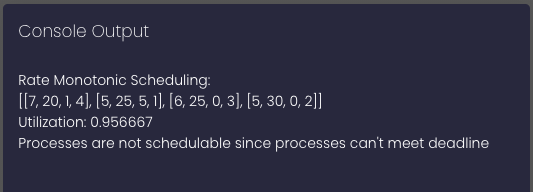
\includegraphics[width=9cm, height=3cm]{Console2.png}}
\caption{Console Log - Input II}
\label{console2}
\end{figure}


\begin{figure}
\centerline{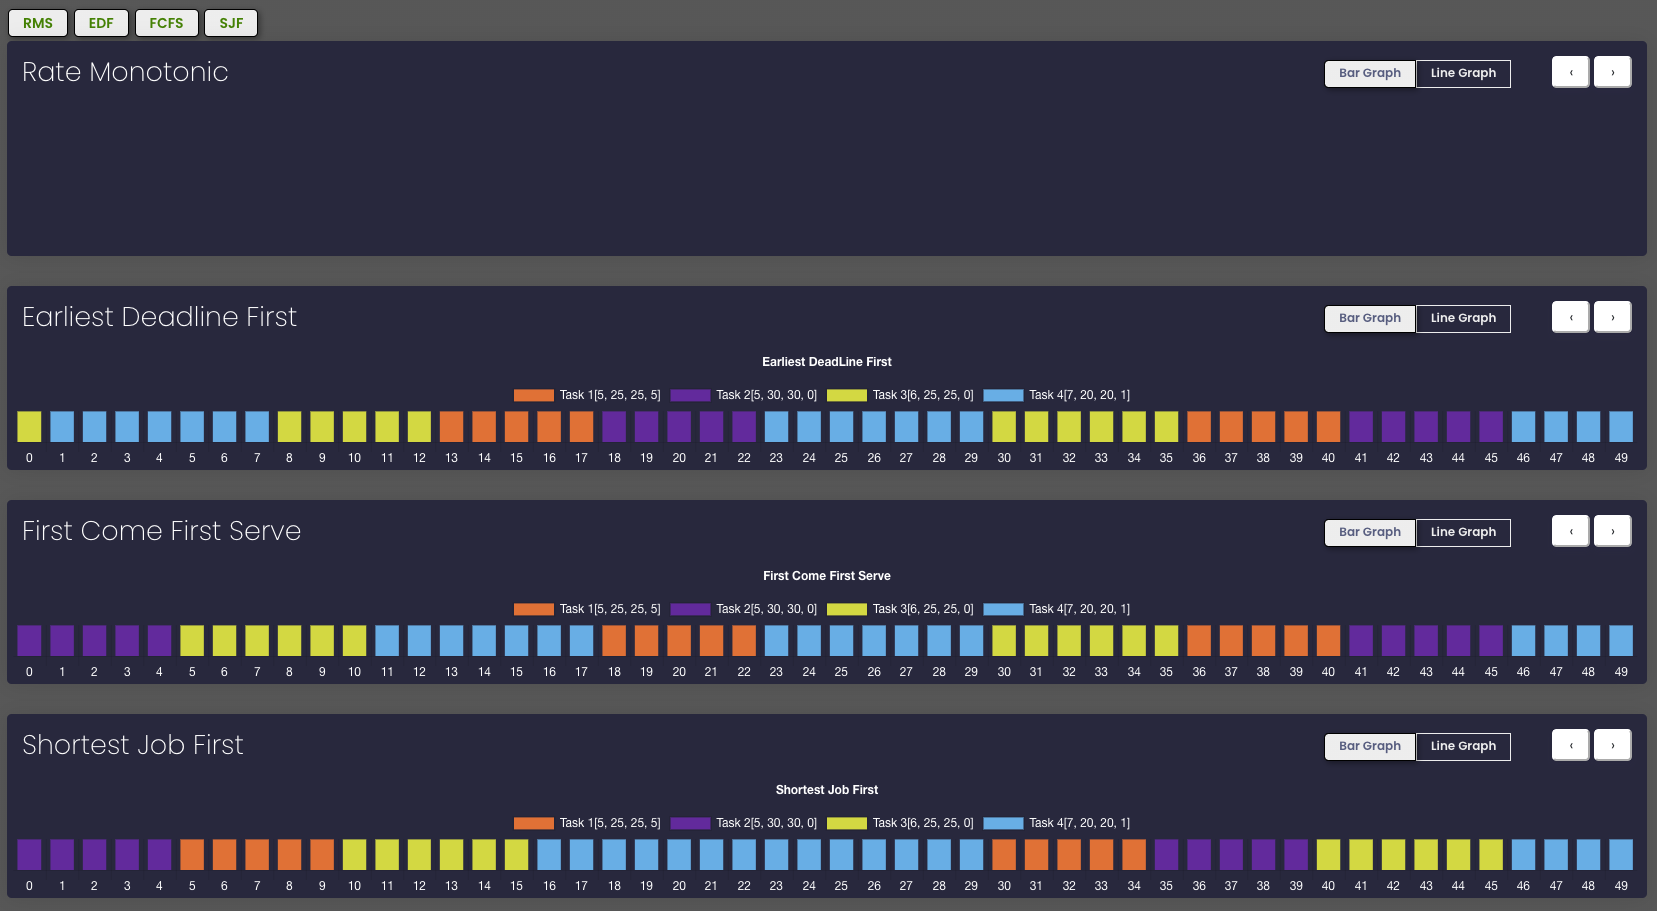
\includegraphics[width=9cm, height=7cm]{Result2.png}}
\caption{Comparison of different scheduling algorithms - Input II}
\label{comparison2}
\end{figure}


\section{Conclusion And Future work}
The simulator as expected provides a good overview of how the scheduling algorithms execute and to compare different algorithms. Which can be used as a tool for learning and teaching the basics of scheduling algorithms. For using the Scheduling Simulator one does not have to know the technical aspects of the application, and also with features provided for easy use of the application and also the interaction with it makes the application intuitive. \\
Future work would mainly focus on expanding the application by including more scheduling algorithms for simulation.  Also, provide an option to save the inputs from the table available on the screen.


\begin{thebibliography}{00}
\bibitem{b1} A. S. Pillai and T. B. Isha, "A new real time simulator for task scheduling," 2012 IEEE International Conference on Computational Intelligence and Computing Research, Coimbatore, 2012, pp. 1-4, doi: 10.1109/ICCIC.2012.6510232.
\bibitem{b2} Chart.js https://www.chartjs.org/ Accessed: 22.08.2020
\bibitem{b3} Black Dashboard https://www.creative-tim.com/product/black-dashboard Accessed: 22.08.2020
\bibitem{b4} Dragos-Paul Pop, Adam Altar, "Designing an MVC Model for Rapid Web Application Development" Procedia Engineering, Volume 69, 2014, Pages 1172-1179, ISSN 1877-7058.
\bibitem{b5}E. Okuyan and B. Kayayurt, "Earliest deadline first scheduling algorithm and its use in ANKA UAV," 2012 IEEE/AIAA 31st Digital Avionics Systems Conference (DASC), Williamsburg, VA, 2012, pp. 8B1-1-8B1-8, doi: 10.1109/DASC.2012.6382435.
\bibitem{b6}M. Saleh and L. Dong, "Comparing FCFS \& EDF scheduling algorithms for real-time packet switching networks," 2010 International Conference on Networking, Sensing and Control (ICNSC), Chicago, IL, 2010, pp. 698-703, doi: 10.1109/ICNSC.2010.5461572.
\bibitem{b7} Lui Sha, R. Rajkumar and S. S. Sathaye, "Generalized rate-monotonic scheduling theory: a framework for developing real-time systems," in Proceedings of the IEEE, vol. 82, no. 1, pp. 68-82, Jan. 1994, doi: 10.1109/5.259427.
\bibitem{b8} https://www.geeksforgeeks.org/program-for-shortest-job-first-or-sjf-cpu-scheduling-set-1-non-preemptive/
\bibitem{b9} Module 6 Embedded System Software, https://nptel.ac.in/content/storage2/courses/108105057/Pdf/Lesson-30.pdf Accessed: 25.08.2020
\end{thebibliography}
\vspace{12pt}

\end{document}
